% Options for packages loaded elsewhere
% Options for packages loaded elsewhere
\PassOptionsToPackage{unicode}{hyperref}
\PassOptionsToPackage{hyphens}{url}
\PassOptionsToPackage{dvipsnames,svgnames,x11names}{xcolor}
%
\documentclass[
  spanish,
  letterpaper,
  DIV=11,
  numbers=noendperiod]{scrartcl}
\usepackage{xcolor}
\usepackage{amsmath,amssymb}
\setcounter{secnumdepth}{-\maxdimen} % remove section numbering
\usepackage{iftex}
\ifPDFTeX
  \usepackage[T1]{fontenc}
  \usepackage[utf8]{inputenc}
  \usepackage{textcomp} % provide euro and other symbols
\else % if luatex or xetex
  \usepackage{unicode-math} % this also loads fontspec
  \defaultfontfeatures{Scale=MatchLowercase}
  \defaultfontfeatures[\rmfamily]{Ligatures=TeX,Scale=1}
\fi
\usepackage{lmodern}
\ifPDFTeX\else
  % xetex/luatex font selection
\fi
% Use upquote if available, for straight quotes in verbatim environments
\IfFileExists{upquote.sty}{\usepackage{upquote}}{}
\IfFileExists{microtype.sty}{% use microtype if available
  \usepackage[]{microtype}
  \UseMicrotypeSet[protrusion]{basicmath} % disable protrusion for tt fonts
}{}
\makeatletter
\@ifundefined{KOMAClassName}{% if non-KOMA class
  \IfFileExists{parskip.sty}{%
    \usepackage{parskip}
  }{% else
    \setlength{\parindent}{0pt}
    \setlength{\parskip}{6pt plus 2pt minus 1pt}}
}{% if KOMA class
  \KOMAoptions{parskip=half}}
\makeatother
% Make \paragraph and \subparagraph free-standing
\makeatletter
\ifx\paragraph\undefined\else
  \let\oldparagraph\paragraph
  \renewcommand{\paragraph}{
    \@ifstar
      \xxxParagraphStar
      \xxxParagraphNoStar
  }
  \newcommand{\xxxParagraphStar}[1]{\oldparagraph*{#1}\mbox{}}
  \newcommand{\xxxParagraphNoStar}[1]{\oldparagraph{#1}\mbox{}}
\fi
\ifx\subparagraph\undefined\else
  \let\oldsubparagraph\subparagraph
  \renewcommand{\subparagraph}{
    \@ifstar
      \xxxSubParagraphStar
      \xxxSubParagraphNoStar
  }
  \newcommand{\xxxSubParagraphStar}[1]{\oldsubparagraph*{#1}\mbox{}}
  \newcommand{\xxxSubParagraphNoStar}[1]{\oldsubparagraph{#1}\mbox{}}
\fi
\makeatother

\usepackage{color}
\usepackage{fancyvrb}
\newcommand{\VerbBar}{|}
\newcommand{\VERB}{\Verb[commandchars=\\\{\}]}
\DefineVerbatimEnvironment{Highlighting}{Verbatim}{commandchars=\\\{\}}
% Add ',fontsize=\small' for more characters per line
\usepackage{framed}
\definecolor{shadecolor}{RGB}{241,243,245}
\newenvironment{Shaded}{\begin{snugshade}}{\end{snugshade}}
\newcommand{\AlertTok}[1]{\textcolor[rgb]{0.68,0.00,0.00}{#1}}
\newcommand{\AnnotationTok}[1]{\textcolor[rgb]{0.37,0.37,0.37}{#1}}
\newcommand{\AttributeTok}[1]{\textcolor[rgb]{0.40,0.45,0.13}{#1}}
\newcommand{\BaseNTok}[1]{\textcolor[rgb]{0.68,0.00,0.00}{#1}}
\newcommand{\BuiltInTok}[1]{\textcolor[rgb]{0.00,0.23,0.31}{#1}}
\newcommand{\CharTok}[1]{\textcolor[rgb]{0.13,0.47,0.30}{#1}}
\newcommand{\CommentTok}[1]{\textcolor[rgb]{0.37,0.37,0.37}{#1}}
\newcommand{\CommentVarTok}[1]{\textcolor[rgb]{0.37,0.37,0.37}{\textit{#1}}}
\newcommand{\ConstantTok}[1]{\textcolor[rgb]{0.56,0.35,0.01}{#1}}
\newcommand{\ControlFlowTok}[1]{\textcolor[rgb]{0.00,0.23,0.31}{\textbf{#1}}}
\newcommand{\DataTypeTok}[1]{\textcolor[rgb]{0.68,0.00,0.00}{#1}}
\newcommand{\DecValTok}[1]{\textcolor[rgb]{0.68,0.00,0.00}{#1}}
\newcommand{\DocumentationTok}[1]{\textcolor[rgb]{0.37,0.37,0.37}{\textit{#1}}}
\newcommand{\ErrorTok}[1]{\textcolor[rgb]{0.68,0.00,0.00}{#1}}
\newcommand{\ExtensionTok}[1]{\textcolor[rgb]{0.00,0.23,0.31}{#1}}
\newcommand{\FloatTok}[1]{\textcolor[rgb]{0.68,0.00,0.00}{#1}}
\newcommand{\FunctionTok}[1]{\textcolor[rgb]{0.28,0.35,0.67}{#1}}
\newcommand{\ImportTok}[1]{\textcolor[rgb]{0.00,0.46,0.62}{#1}}
\newcommand{\InformationTok}[1]{\textcolor[rgb]{0.37,0.37,0.37}{#1}}
\newcommand{\KeywordTok}[1]{\textcolor[rgb]{0.00,0.23,0.31}{\textbf{#1}}}
\newcommand{\NormalTok}[1]{\textcolor[rgb]{0.00,0.23,0.31}{#1}}
\newcommand{\OperatorTok}[1]{\textcolor[rgb]{0.37,0.37,0.37}{#1}}
\newcommand{\OtherTok}[1]{\textcolor[rgb]{0.00,0.23,0.31}{#1}}
\newcommand{\PreprocessorTok}[1]{\textcolor[rgb]{0.68,0.00,0.00}{#1}}
\newcommand{\RegionMarkerTok}[1]{\textcolor[rgb]{0.00,0.23,0.31}{#1}}
\newcommand{\SpecialCharTok}[1]{\textcolor[rgb]{0.37,0.37,0.37}{#1}}
\newcommand{\SpecialStringTok}[1]{\textcolor[rgb]{0.13,0.47,0.30}{#1}}
\newcommand{\StringTok}[1]{\textcolor[rgb]{0.13,0.47,0.30}{#1}}
\newcommand{\VariableTok}[1]{\textcolor[rgb]{0.07,0.07,0.07}{#1}}
\newcommand{\VerbatimStringTok}[1]{\textcolor[rgb]{0.13,0.47,0.30}{#1}}
\newcommand{\WarningTok}[1]{\textcolor[rgb]{0.37,0.37,0.37}{\textit{#1}}}

\usepackage{longtable,booktabs,array}
\usepackage{calc} % for calculating minipage widths
% Correct order of tables after \paragraph or \subparagraph
\usepackage{etoolbox}
\makeatletter
\patchcmd\longtable{\par}{\if@noskipsec\mbox{}\fi\par}{}{}
\makeatother
% Allow footnotes in longtable head/foot
\IfFileExists{footnotehyper.sty}{\usepackage{footnotehyper}}{\usepackage{footnote}}
\makesavenoteenv{longtable}
\usepackage{graphicx}
\makeatletter
\newsavebox\pandoc@box
\newcommand*\pandocbounded[1]{% scales image to fit in text height/width
  \sbox\pandoc@box{#1}%
  \Gscale@div\@tempa{\textheight}{\dimexpr\ht\pandoc@box+\dp\pandoc@box\relax}%
  \Gscale@div\@tempb{\linewidth}{\wd\pandoc@box}%
  \ifdim\@tempb\p@<\@tempa\p@\let\@tempa\@tempb\fi% select the smaller of both
  \ifdim\@tempa\p@<\p@\scalebox{\@tempa}{\usebox\pandoc@box}%
  \else\usebox{\pandoc@box}%
  \fi%
}
% Set default figure placement to htbp
\def\fps@figure{htbp}
\makeatother



\ifLuaTeX
\usepackage[bidi=basic]{babel}
\else
\usepackage[bidi=default]{babel}
\fi
% get rid of language-specific shorthands (see #6817):
\let\LanguageShortHands\languageshorthands
\def\languageshorthands#1{}


\setlength{\emergencystretch}{3em} % prevent overfull lines

\providecommand{\tightlist}{%
  \setlength{\itemsep}{0pt}\setlength{\parskip}{0pt}}



 


\usepackage{booktabs}
\usepackage{longtable}
\usepackage{array}
\usepackage{multirow}
\usepackage{wrapfig}
\usepackage{float}
\usepackage{colortbl}
\usepackage{pdflscape}
\usepackage{tabu}
\usepackage{threeparttable}
\usepackage{threeparttablex}
\usepackage[normalem]{ulem}
\usepackage{makecell}
\usepackage{xcolor}
\KOMAoption{captions}{tableheading}
\makeatletter
\@ifpackageloaded{caption}{}{\usepackage{caption}}
\AtBeginDocument{%
\ifdefined\contentsname
  \renewcommand*\contentsname{Tabla de contenidos}
\else
  \newcommand\contentsname{Tabla de contenidos}
\fi
\ifdefined\listfigurename
  \renewcommand*\listfigurename{Listado de Figuras}
\else
  \newcommand\listfigurename{Listado de Figuras}
\fi
\ifdefined\listtablename
  \renewcommand*\listtablename{Listado de Tablas}
\else
  \newcommand\listtablename{Listado de Tablas}
\fi
\ifdefined\figurename
  \renewcommand*\figurename{Figura}
\else
  \newcommand\figurename{Figura}
\fi
\ifdefined\tablename
  \renewcommand*\tablename{Tabla}
\else
  \newcommand\tablename{Tabla}
\fi
}
\@ifpackageloaded{float}{}{\usepackage{float}}
\floatstyle{ruled}
\@ifundefined{c@chapter}{\newfloat{codelisting}{h}{lop}}{\newfloat{codelisting}{h}{lop}[chapter]}
\floatname{codelisting}{Listado}
\newcommand*\listoflistings{\listof{codelisting}{Listado de Listados}}
\makeatother
\makeatletter
\makeatother
\makeatletter
\@ifpackageloaded{caption}{}{\usepackage{caption}}
\@ifpackageloaded{subcaption}{}{\usepackage{subcaption}}
\makeatother
\usepackage{bookmark}
\IfFileExists{xurl.sty}{\usepackage{xurl}}{} % add URL line breaks if available
\urlstyle{same}
\hypersetup{
  pdftitle={TP final de Regresión Avanzada},
  pdfauthor={Martín Ceriotti},
  pdflang={es},
  colorlinks=true,
  linkcolor={blue},
  filecolor={Maroon},
  citecolor={Blue},
  urlcolor={Blue},
  pdfcreator={LaTeX via pandoc}}


\title{TP final de Regresión Avanzada}
\author{Martín Ceriotti}
\date{2026-04-22}
\begin{document}
\maketitle


\subsection{Consigna I: Regresión
Lineal}\label{consigna-i-regresiuxf3n-lineal}

\subsubsection{Modelo 1:}\label{modelo-1}

Modelo de Selección Automática por Criterio de Información de Akaike
(AIC). Se busca equilibrio entre bondad de ajuste y complejidad.

\paragraph{Summary del Modelo 1:}\label{summary-del-modelo-1}

\begin{longtable}[t]{lrrrr}
\caption{\label{tab:unnamed-chunk-2}Coeficientes del Modelo AIC}\\
\toprule
\cellcolor{black}{\textcolor{white}{Término}} & \cellcolor{black}{\textcolor{white}{Estimación}} & \cellcolor{black}{\textcolor{white}{Error Est.}} & \cellcolor{black}{\textcolor{white}{Estadístico t}} & \cellcolor{black}{\textcolor{white}{p-valor}}\\
\midrule
(Intercept) & -31.387 & 80.120 & -0.392 & 0.695\\
formalSi & 301.373 & 18.738 & 16.083 & 0.000\\
horas\_trabajo & 10.685 & 0.507 & 21.083 & 0.000\\
educ\_catPrimario & 103.327 & 57.909 & 1.784 & 0.074\\
educ\_catSecundario & 237.627 & 57.295 & 4.147 & 0.000\\
\addlinespace
educ\_catSuperior & 606.553 & 58.631 & 10.345 & 0.000\\
regionGran Buenos Aires & 139.120 & 31.028 & 4.484 & 0.000\\
regionNoreste & -138.258 & 35.808 & -3.861 & 0.000\\
regionNoroeste & -135.490 & 27.324 & -4.959 & 0.000\\
regionPampeana & 92.236 & 27.117 & 3.401 & 0.001\\
\addlinespace
regionPatagonia & 372.126 & 31.397 & 11.852 & 0.000\\
edad & 4.409 & 0.768 & 5.745 & 0.000\\
sexoMujer & -152.074 & 16.042 & -9.480 & 0.000\\
est\_civilseparado o divorciado & -119.809 & 30.625 & -3.912 & 0.000\\
est\_civilsoltero & -137.890 & 21.782 & -6.331 & 0.000\\
\addlinespace
est\_civilunido & -63.006 & 20.973 & -3.004 & 0.003\\
est\_civilviudo & -183.927 & 64.599 & -2.847 & 0.004\\
ant\_laboral1 a 5 años & -23.976 & 38.658 & -0.620 & 0.535\\
ant\_laboral6 meses a 1 año & -81.538 & 49.308 & -1.654 & 0.098\\
ant\_laboralEntre 3 y 6 meses & -52.459 & 52.688 & -0.996 & 0.319\\
\addlinespace
ant\_laboralMas de 5 años & 43.689 & 39.919 & 1.094 & 0.274\\
ant\_laboralMenos de 1 mes & -92.420 & 84.885 & -1.089 & 0.276\\
\bottomrule
\end{longtable}

\subsubsection{Modelo 2:}\label{modelo-2}

Modelo de Selección Automática por Criterio de Información Bayesiano
(BIC). Este modelo se seleccionó bajo el principio de parsimonia.

\paragraph{Summary del Modelo 2:}\label{summary-del-modelo-2}

\begin{longtable}[t]{lrrrr}
\caption{\label{tab:unnamed-chunk-3}Coeficientes del Modelo BIC}\\
\toprule
\cellcolor{black}{\textcolor{white}{Término}} & \cellcolor{black}{\textcolor{white}{Estimación}} & \cellcolor{black}{\textcolor{white}{Error Est.}} & \cellcolor{black}{\textcolor{white}{Estadístico t}} & \cellcolor{black}{\textcolor{white}{p-valor}}\\
\midrule
(Intercept) & -96.008 & 72.845 & -1.318 & 0.188\\
formalSi & 325.312 & 17.701 & 18.378 & 0.000\\
horas\_trabajo & 10.682 & 0.507 & 21.089 & 0.000\\
educ\_catPrimario & 114.441 & 57.823 & 1.979 & 0.048\\
educ\_catSecundario & 249.276 & 57.209 & 4.357 & 0.000\\
\addlinespace
educ\_catSuperior & 618.675 & 58.515 & 10.573 & 0.000\\
regionGran Buenos Aires & 135.205 & 31.050 & 4.354 & 0.000\\
regionNoreste & -134.968 & 35.839 & -3.766 & 0.000\\
regionNoroeste & -134.538 & 27.352 & -4.919 & 0.000\\
regionPampeana & 89.017 & 27.131 & 3.281 & 0.001\\
\addlinespace
regionPatagonia & 370.224 & 31.425 & 11.781 & 0.000\\
edad & 5.661 & 0.710 & 7.974 & 0.000\\
sexoMujer & -151.990 & 16.054 & -9.468 & 0.000\\
est\_civilseparado o divorciado & -124.849 & 30.628 & -4.076 & 0.000\\
est\_civilsoltero & -144.305 & 21.744 & -6.636 & 0.000\\
\addlinespace
est\_civilunido & -63.584 & 20.978 & -3.031 & 0.002\\
est\_civilviudo & -195.632 & 64.621 & -3.027 & 0.002\\
\bottomrule
\end{longtable}

\subsubsection{Modelo 3:}\label{modelo-3}

En teoría la instrucción y la experiencia son los motores principales de
la productividad, por ende, del salario. Es por esto que elegí las
variables educ\_cat, horas\_trabajo y formal como explicativas del
ingreso\_ocup.

\paragraph{Summary del Modelo 3:}\label{summary-del-modelo-3}

\begin{longtable}[t]{lrrrr}
\caption{\label{tab:unnamed-chunk-4}Coeficientes del Modelo Propio}\\
\toprule
\cellcolor{black}{\textcolor{white}{Término}} & \cellcolor{black}{\textcolor{white}{Estimación}} & \cellcolor{black}{\textcolor{white}{Error Est.}} & \cellcolor{black}{\textcolor{white}{Estadístico t}} & \cellcolor{black}{\textcolor{white}{p-valor}}\\
\midrule
(Intercept) & -46.625 & 62.464 & -0.746 & 0.455\\
educ\_catPrimario & 100.630 & 60.958 & 1.651 & 0.099\\
educ\_catSecundario & 169.447 & 60.003 & 2.824 & 0.005\\
educ\_catSuperior & 523.156 & 61.284 & 8.537 & 0.000\\
horas\_trabajo & 12.274 & 0.518 & 23.676 & 0.000\\
\addlinespace
formalSi & 447.041 & 17.682 & 25.282 & 0.000\\
\bottomrule
\end{longtable}

\subsubsection{Comparación de los
Modelos}\label{comparaciuxf3n-de-los-modelos}

\begin{Shaded}
\begin{Highlighting}[]
\CommentTok{\# 3. Comparar los 3 modelos a través de las siguientes métricas de performance: CME, PRESS, AIC y BIC. En base a los resultados observados, elegir un modelo “ganador”.}

\NormalTok{criterios }\OtherTok{\textless{}{-}} \ControlFlowTok{function}\NormalTok{(m, maxi) \{}
  
\NormalTok{  SCE }\OtherTok{\textless{}{-}} \FunctionTok{deviance}\NormalTok{(m)}
\NormalTok{  n }\OtherTok{\textless{}{-}} \FunctionTok{length}\NormalTok{(}\FunctionTok{residuals}\NormalTok{(m))}
\NormalTok{  p }\OtherTok{\textless{}{-}} \FunctionTok{length}\NormalTok{(}\FunctionTok{coefficients}\NormalTok{(m)) }\CommentTok{\#incluye intercepto}
  
  \CommentTok{\#CME}
\NormalTok{  cme }\OtherTok{\textless{}{-}}\NormalTok{ SCE}\SpecialCharTok{/}\NormalTok{(n}\SpecialCharTok{{-}}\NormalTok{p)}
  
  \CommentTok{\#R2 ajustado}
\NormalTok{  r2aj }\OtherTok{\textless{}{-}} \FunctionTok{summary}\NormalTok{(m)}\SpecialCharTok{$}\NormalTok{adj.r.squared}
  
  \CommentTok{\#AKAIKE}
\NormalTok{  akaike }\OtherTok{\textless{}{-}} \FunctionTok{AIC}\NormalTok{(m)}
  
  \CommentTok{\#BIC}
\NormalTok{  schwarz }\OtherTok{\textless{}{-}} \FunctionTok{BIC}\NormalTok{(m)}
  
  \FunctionTok{tibble}\NormalTok{(}\AttributeTok{CME =}\NormalTok{ cme, }\AttributeTok{R2Aj =}\NormalTok{ r2aj, }\AttributeTok{AIC =}\NormalTok{ akaike, }\AttributeTok{BIC =}\NormalTok{ schwarz)}
\NormalTok{\}}

\FunctionTok{map\_dfr}\NormalTok{(}\FunctionTok{list}\NormalTok{(mod\_aic, mod\_baic, mod\_propio), criterios, }\AttributeTok{maxi =}\NormalTok{ mod\_aic) }\SpecialCharTok{\%\textgreater{}\%} 
  \FunctionTok{mutate\_all}\NormalTok{(round, }\DecValTok{4}\NormalTok{) }\SpecialCharTok{\%\textgreater{}\%} 
  \FunctionTok{mutate}\NormalTok{(}
    \AttributeTok{Modelo =} \FunctionTok{c}\NormalTok{(}\StringTok{"Mod AIC"}\NormalTok{, }\StringTok{"Mod BAIC"}\NormalTok{, }\StringTok{"Modelo Propio"}\NormalTok{),}
    \AttributeTok{Explicativas =} \FunctionTok{c}\NormalTok{(}
      \StringTok{"sexo + edad + est\_civil +region+ horas\_trabajo +educ\_cat + formal + ant\_laboral"}\NormalTok{,}
      \StringTok{"sexo + edad + est\_civil +region+ horas\_trabajo +educ\_cat + formal + ant\_laboral"}\NormalTok{,}
      \StringTok{"educ\_cat + horas\_trabajo + formal"}
\NormalTok{    )}
\NormalTok{  ) }\SpecialCharTok{\%\textgreater{}\%} 
\NormalTok{  dplyr}\SpecialCharTok{::}\FunctionTok{select}\NormalTok{(Modelo, Explicativas, CME, }\StringTok{"$R\_\{aj\}\^{}2$"} \OtherTok{=}\NormalTok{ R2Aj, AIC, BIC) }\SpecialCharTok{\%\textgreater{}\%} 
  \FunctionTok{kable}\NormalTok{(}\AttributeTok{escape =} \ConstantTok{FALSE}\NormalTok{) }\SpecialCharTok{\%\textgreater{}\%} 
  \FunctionTok{kable\_styling}\NormalTok{(}\AttributeTok{full\_width =}\NormalTok{ F) }\SpecialCharTok{\%\textgreater{}\%} 
  \FunctionTok{row\_spec}\NormalTok{(}\DecValTok{0}\NormalTok{, }\AttributeTok{background =} \StringTok{"black"}\NormalTok{, }\AttributeTok{color =} \StringTok{"white"}\NormalTok{, }\AttributeTok{bold =}\NormalTok{ T) }\SpecialCharTok{\%\textgreater{}\%} 
  \FunctionTok{row\_spec}\NormalTok{(}\DecValTok{1}\NormalTok{, }\AttributeTok{background =} \StringTok{"\#A9F5A9"}\NormalTok{) }\SpecialCharTok{\%\textgreater{}\%} 
  \FunctionTok{row\_spec}\NormalTok{(}\DecValTok{2}\NormalTok{, }\AttributeTok{background =} \StringTok{"\#A9D0F5"}\NormalTok{) }\SpecialCharTok{\%\textgreater{}\%} 
  \FunctionTok{row\_spec}\NormalTok{(}\DecValTok{3}\NormalTok{, }\AttributeTok{background =} \StringTok{"\#F5A9A9"}\NormalTok{)}
\end{Highlighting}
\end{Shaded}

\begin{longtable*}[t]{llrrrr}
\toprule
\cellcolor{black}{\textcolor{white}{\textbf{Modelo}}} & \cellcolor{black}{\textcolor{white}{\textbf{Explicativas}}} & \cellcolor{black}{\textcolor{white}{\textbf{CME}}} & \cellcolor{black}{\textcolor{white}{\textbf{\$R\_\{aj\}\textasciicircum{}2\$}}} & \cellcolor{black}{\textcolor{white}{\textbf{AIC}}} & \cellcolor{black}{\textcolor{white}{\textbf{BIC}}}\\
\midrule
\cellcolor[HTML]{A9F5A9}{Mod AIC} & \cellcolor[HTML]{A9F5A9}{sexo + edad + est\_civil +region+ horas\_trabajo +educ\_cat + formal + ant\_laboral} & \cellcolor[HTML]{A9F5A9}{339165.3} & \cellcolor[HTML]{A9F5A9}{0.3273} & \cellcolor[HTML]{A9F5A9}{100059.3} & \cellcolor[HTML]{A9F5A9}{100214.9}\\
\cellcolor[HTML]{A9D0F5}{Mod BAIC} & \cellcolor[HTML]{A9D0F5}{sexo + edad + est\_civil +region+ horas\_trabajo +educ\_cat + formal + ant\_laboral} & \cellcolor[HTML]{A9D0F5}{340028.6} & \cellcolor[HTML]{A9D0F5}{0.3256} & \cellcolor[HTML]{A9D0F5}{100070.6} & \cellcolor[HTML]{A9D0F5}{100192.4}\\
\cellcolor[HTML]{F5A9A9}{Modelo Propio} & \cellcolor[HTML]{F5A9A9}{educ\_cat + horas\_trabajo + formal} & \cellcolor[HTML]{F5A9A9}{379610.7} & \cellcolor[HTML]{F5A9A9}{0.2471} & \cellcolor[HTML]{F5A9A9}{100767.0} & \cellcolor[HTML]{F5A9A9}{100814.4}\\
\bottomrule
\end{longtable*}

El modelo mod\_aic destaca en 3 de los 4 indicadores. Podemos concluir
que es el modelo ganador.

\subsubsection{Análisis de Residuos}\label{anuxe1lisis-de-residuos}

\begin{Shaded}
\begin{Highlighting}[]
\CommentTok{\# {-}{-}{-} A. Linealidad y Homocedasticidad {-}{-}{-}}
\FunctionTok{plot}\NormalTok{(mod\_aic, }\DecValTok{1}\NormalTok{) }\CommentTok{\# Gráfico: Valores Ajustados vs Residuos}
\end{Highlighting}
\end{Shaded}

\pandocbounded{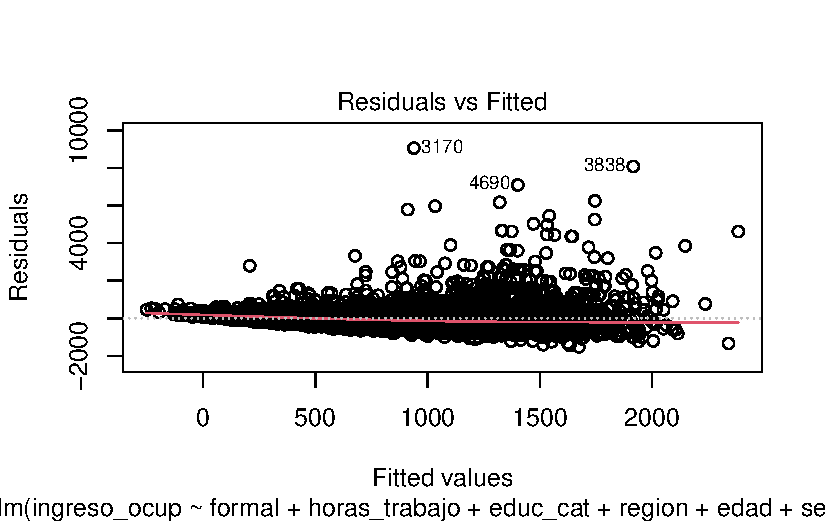
\includegraphics[keepaspectratio]{index_files/figure-pdf/unnamed-chunk-6-1.pdf}}

\begin{Shaded}
\begin{Highlighting}[]
\FunctionTok{bptest}\NormalTok{(mod\_aic)  }\CommentTok{\# Test de Breusch{-}Pagan (H0: Homocedasticidad)}
\end{Highlighting}
\end{Shaded}

\begin{verbatim}

    studentized Breusch-Pagan test

data:  mod_aic
BP = 146.22, df = 21, p-value < 2.2e-16
\end{verbatim}

Gráfico Residuals vs Fitted: La varianza de los residuos aumenta
claramente con los valores ajustados (forma de abanico) → indica
heterocedasticidad.

Breusch-Pagan: BP = 146.22, p-value \textless{} 2.2e-16 → Se rechaza H0
→ Se confirma heterocedasticidad. El supuesto no se cumple.

\begin{Shaded}
\begin{Highlighting}[]
\CommentTok{\# {-}{-}{-} B. Normalidad {-}{-}{-}}
\FunctionTok{plot}\NormalTok{(mod\_aic, }\DecValTok{2}\NormalTok{) }\CommentTok{\# Gráfico: QQ{-}Plot}
\end{Highlighting}
\end{Shaded}

\pandocbounded{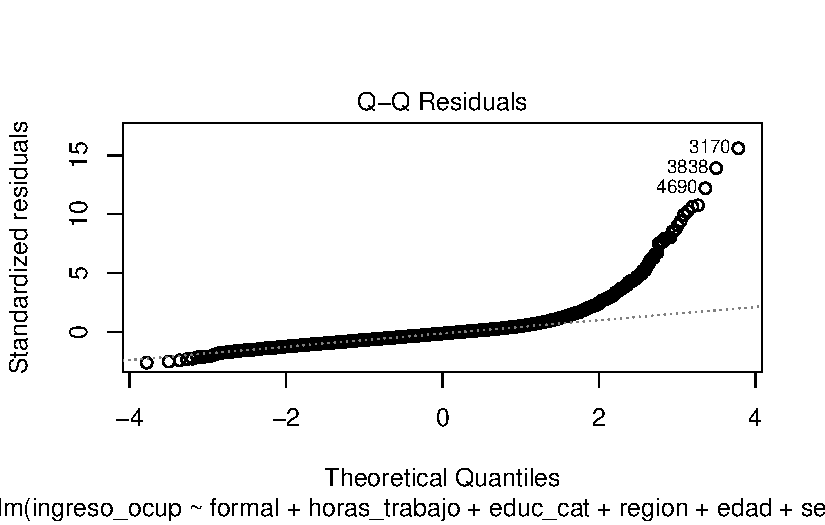
\includegraphics[keepaspectratio]{index_files/figure-pdf/unnamed-chunk-7-1.pdf}}

\begin{Shaded}
\begin{Highlighting}[]
\FunctionTok{ad.test}\NormalTok{(}\FunctionTok{residuals}\NormalTok{(mod\_aic)) }\CommentTok{\# Test de Anderson{-}Darling (H0: Normalidad)}
\end{Highlighting}
\end{Shaded}

\begin{verbatim}

    Anderson-Darling normality test

data:  residuals(mod_aic)
A = 316.49, p-value < 2.2e-16
\end{verbatim}

\begin{Shaded}
\begin{Highlighting}[]
\CommentTok{\#QQ{-}Plot: Los residuos se desvían fuertemente de la línea teórica, especialmente en la cola derecha → no hay normalidad.}
\CommentTok{\#Anderson{-}Darling: A = 316.49, p{-}value \textless{} 2.2e{-}16 → Se rechaza H0 → Se confirma no normalidad. El supuesto no se cumple.}
\end{Highlighting}
\end{Shaded}

\begin{Shaded}
\begin{Highlighting}[]
\CommentTok{\# {-}{-}{-} C. Independencia de los Errores {-}{-}{-}}
\FunctionTok{dwtest}\NormalTok{(mod\_aic) }\CommentTok{\# Test de Durbin{-}Watson (H0: Autocorrelación nula)}
\end{Highlighting}
\end{Shaded}

\begin{verbatim}

    Durbin-Watson test

data:  mod_aic
DW = 1.8716, p-value = 1.127e-07
alternative hypothesis: true autocorrelation is greater than 0
\end{verbatim}

\begin{Shaded}
\begin{Highlighting}[]
\CommentTok{\#Durbin{-}Watson: DW = 1.8716, p{-}value = 1.127e{-}07 → Se rechaza H0 → Existe autocorrelación positiva leve. El supuesto no se cumple estrictamente, aunque el DW está cerca de 2.}
\end{Highlighting}
\end{Shaded}

\begin{Shaded}
\begin{Highlighting}[]
\CommentTok{\# {-}{-}{-} D. Multicolinealidad {-}{-}{-}}
\FunctionTok{vif}\NormalTok{(mod\_aic) }\CommentTok{\# Factor de Inflación de la Varianza (Idealmente \textless{} 5)}
\end{Highlighting}
\end{Shaded}

\begin{verbatim}
                  GVIF Df GVIF^(1/(2*Df))
formal        1.425510  1        1.193947
horas_trabajo 1.105217  1        1.051293
educ_cat      1.293037  3        1.043763
region        1.070397  5        1.006826
edad          1.681666  1        1.296791
sexo          1.178648  1        1.085655
est_civil     1.465346  4        1.048920
ant_laboral   1.581460  5        1.046902
\end{verbatim}

\begin{Shaded}
\begin{Highlighting}[]
\CommentTok{\# En general, valores de VIF mayores a 5 se consideran problemáticos. En este caso no tenemos ninguno. }
\CommentTok{\# No hay multicolinealidad problemática. El supuesto se cumple.}

\CommentTok{\# {-}{-}{-} E. Observaciones Influyentes y Atípicas {-}{-}{-}}

\FunctionTok{sort}\NormalTok{(}\FunctionTok{cooks.distance}\NormalTok{(mod\_aic), }\AttributeTok{decreasing =} \ConstantTok{TRUE}\NormalTok{)[}\DecValTok{1}\SpecialCharTok{:}\DecValTok{10}\NormalTok{]}
\end{Highlighting}
\end{Shaded}

\begin{verbatim}
      3170       3838       6348       1244       5129         92       3883 
0.05054404 0.03305971 0.02944246 0.01474650 0.01420343 0.01335017 0.01322749 
      4690       1566       5641 
0.01239769 0.01147810 0.01055640 
\end{verbatim}

\begin{Shaded}
\begin{Highlighting}[]
\CommentTok{\#los 10 mas influyentes.}
\end{Highlighting}
\end{Shaded}

\begin{Shaded}
\begin{Highlighting}[]
\FunctionTok{plot}\NormalTok{(mod\_aic, }\DecValTok{5}\NormalTok{)        }\CommentTok{\# Leverage vs Residuos estandarizados (incluye Cook)}
\end{Highlighting}
\end{Shaded}

\pandocbounded{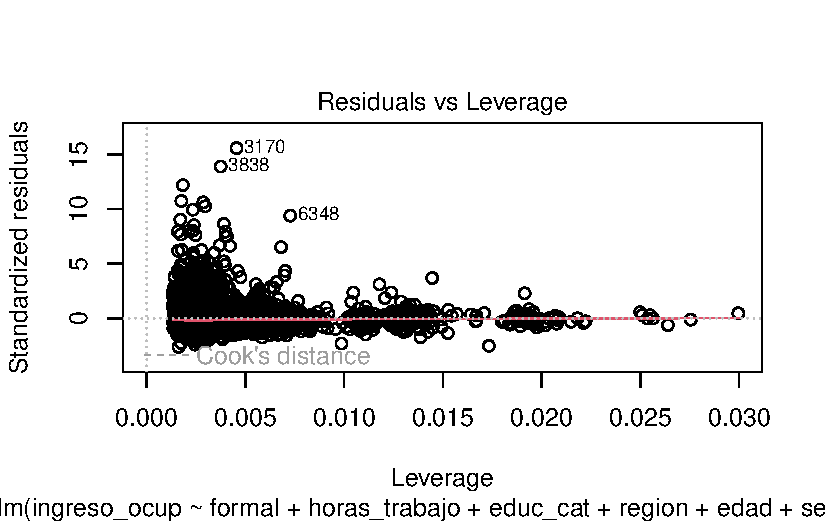
\includegraphics[keepaspectratio]{index_files/figure-pdf/unnamed-chunk-10-1.pdf}}

\begin{Shaded}
\begin{Highlighting}[]
\FunctionTok{influencePlot}\NormalTok{(mod\_aic)  }\CommentTok{\# Tabla con casos influyentes (library(car))}
\end{Highlighting}
\end{Shaded}

\pandocbounded{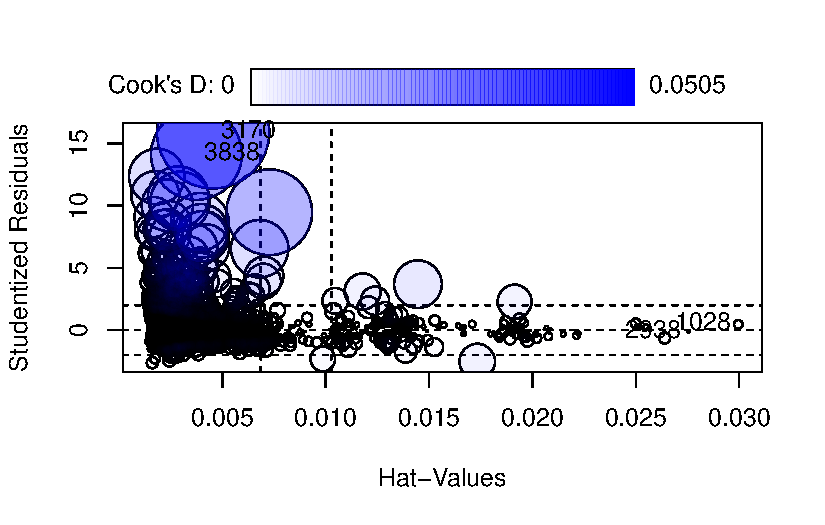
\includegraphics[keepaspectratio]{index_files/figure-pdf/unnamed-chunk-10-2.pdf}}

\begin{verbatim}
        StudRes         Hat        CookD
1028  0.4676938 0.029958512 3.071026e-04
2938 -0.1227876 0.027551609 1.941931e-05
3170 15.8969996 0.004552283 5.054404e-02
3838 14.1210079 0.003746407 3.305971e-02
\end{verbatim}

Running Code

When you click the \textbf{Render} button a document will be generated
that includes both content and the output of embedded code. You can
embed code like this:

\begin{Shaded}
\begin{Highlighting}[]
\NormalTok{criterios }\OtherTok{\textless{}{-}} \ControlFlowTok{function}\NormalTok{(m) \{}
\NormalTok{  SCE }\OtherTok{\textless{}{-}} \FunctionTok{deviance}\NormalTok{(m)}
\NormalTok{  n }\OtherTok{\textless{}{-}} \FunctionTok{length}\NormalTok{(}\FunctionTok{residuals}\NormalTok{(m))}
\NormalTok{  p }\OtherTok{\textless{}{-}} \FunctionTok{length}\NormalTok{(}\FunctionTok{coefficients}\NormalTok{(m))}
\NormalTok{  cme }\OtherTok{\textless{}{-}}\NormalTok{ SCE}\SpecialCharTok{/}\NormalTok{(n}\SpecialCharTok{{-}}\NormalTok{p)}
\NormalTok{  r2aj }\OtherTok{\textless{}{-}} \FunctionTok{summary}\NormalTok{(m)}\SpecialCharTok{$}\NormalTok{adj.r.squared}
  \FunctionTok{tibble}\NormalTok{(}\AttributeTok{CME =}\NormalTok{ cme, }\AttributeTok{R2Aj =}\NormalTok{ r2aj, }\AttributeTok{AIC =} \FunctionTok{AIC}\NormalTok{(m), }\AttributeTok{BIC =} \FunctionTok{BIC}\NormalTok{(m))}
\NormalTok{\}}

\FunctionTok{map\_dfr}\NormalTok{(}\FunctionTok{list}\NormalTok{(mod\_aic, mod\_baic, mod\_propio), criterios) }\SpecialCharTok{\%\textgreater{}\%} 
  \FunctionTok{mutate\_all}\NormalTok{(round, }\DecValTok{2}\NormalTok{) }\SpecialCharTok{\%\textgreater{}\%} 
  \FunctionTok{mutate}\NormalTok{(}\AttributeTok{Modelo =} \FunctionTok{c}\NormalTok{(}\StringTok{"Mod AIC"}\NormalTok{, }\StringTok{"Mod BAIC"}\NormalTok{, }\StringTok{"Modelo Propio"}\NormalTok{)) }\SpecialCharTok{\%\textgreater{}\%} 
\NormalTok{  dplyr}\SpecialCharTok{::}\FunctionTok{select}\NormalTok{(Modelo, CME, }\StringTok{"$R\_\{aj\}\^{}2$"} \OtherTok{=}\NormalTok{ R2Aj, AIC, BIC) }\SpecialCharTok{\%\textgreater{}\%} 
  \FunctionTok{kable}\NormalTok{(}\AttributeTok{escape =} \ConstantTok{FALSE}\NormalTok{, }\AttributeTok{caption =} \StringTok{"Comparación de métricas de ajuste"}\NormalTok{) }\SpecialCharTok{\%\textgreater{}\%} 
  \FunctionTok{kable\_styling}\NormalTok{(}\AttributeTok{full\_width =}\NormalTok{ F, }\AttributeTok{latex\_options =} \StringTok{"hold\_position"}\NormalTok{) }\SpecialCharTok{\%\textgreater{}\%} 
  \FunctionTok{row\_spec}\NormalTok{(}\DecValTok{1}\NormalTok{, }\AttributeTok{background =} \StringTok{"\#A9F5A9"}\NormalTok{)}
\end{Highlighting}
\end{Shaded}

\begin{longtable}[t]{lrrrr}
\caption{\label{tab:unnamed-chunk-11}Comparación de métricas de ajuste}\\
\toprule
Modelo & CME & \$R\_\{aj\}\textasciicircum{}2\$ & AIC & BIC\\
\midrule
\cellcolor[HTML]{A9F5A9}{Mod AIC} & \cellcolor[HTML]{A9F5A9}{339165.3} & \cellcolor[HTML]{A9F5A9}{0.33} & \cellcolor[HTML]{A9F5A9}{100059.3} & \cellcolor[HTML]{A9F5A9}{100214.9}\\
Mod BAIC & 340028.6 & 0.33 & 100070.6 & 100192.4\\
Modelo Propio & 379610.7 & 0.25 & 100767.0 & 100814.4\\
\bottomrule
\end{longtable}

\begin{Shaded}
\begin{Highlighting}[]
\FunctionTok{plot}\NormalTok{(mod\_aic, }\DecValTok{1}\NormalTok{)}
\FunctionTok{plot}\NormalTok{(mod\_aic, }\DecValTok{2}\NormalTok{)}
\end{Highlighting}
\end{Shaded}

\begin{figure}

\begin{minipage}{0.50\linewidth}
\pandocbounded{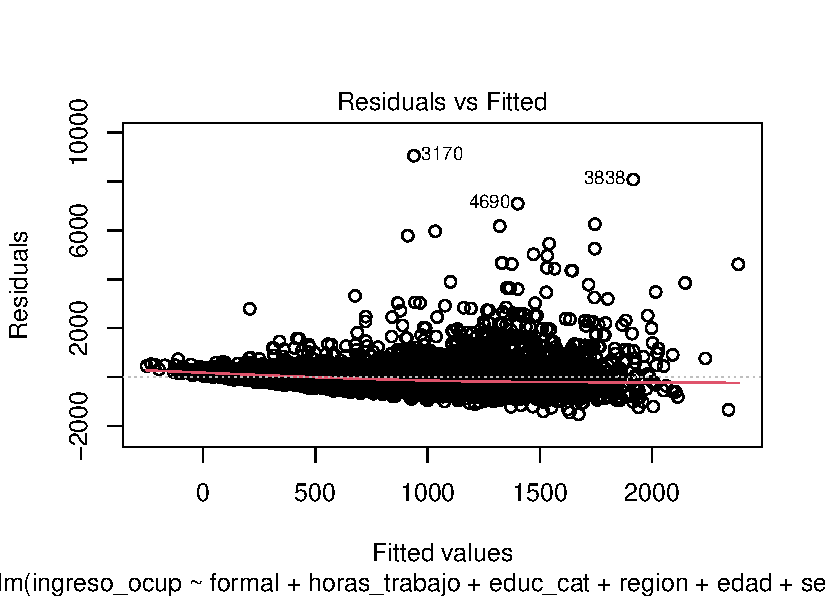
\includegraphics[keepaspectratio]{index_files/figure-pdf/unnamed-chunk-12-1.pdf}}\end{minipage}%
%
\begin{minipage}{0.50\linewidth}
\pandocbounded{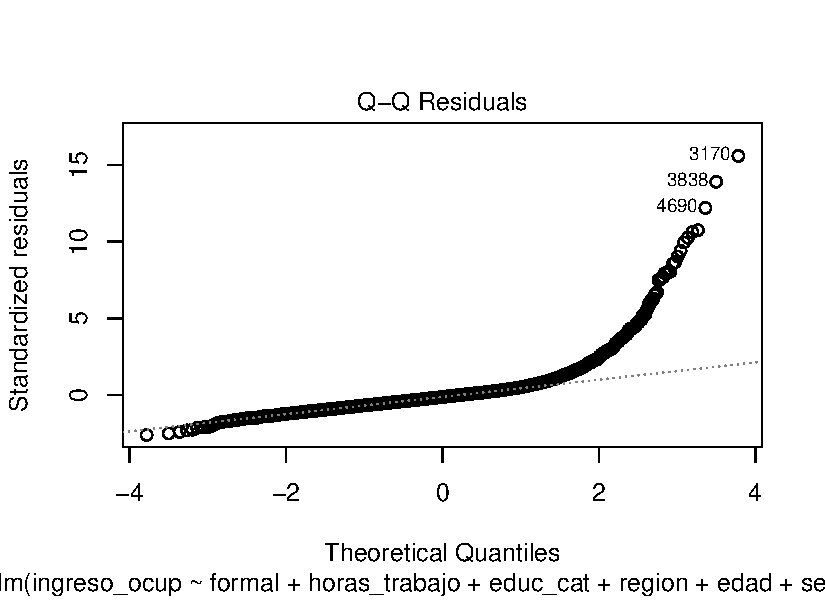
\includegraphics[keepaspectratio]{index_files/figure-pdf/unnamed-chunk-12-2.pdf}}\end{minipage}%

\end{figure}%

You can add options to executable code like this

The \texttt{echo:\ false} option disables the printing of code (only
output is displayed).




\end{document}
